%%%%%%%%%%%%%%%%%%%%%%%%%%%%%%%%%%%%%%%%%%%%%%%%%%%%%%%%%%%
% --------------------------------------------------------
% Tau
% LaTeX Template
% Version 2.4.1 (22/05/2024)
%
% Author: 
% Guillermo Jimenez (memo.notess1@gmail.com)
% 
% License:
% Creative Commons CC BY 4.0
% --------------------------------------------------------
%%%%%%%%%%%%%%%%%%%%%%%%%%%%%%%%%%%%%%%%%%%%%%%%%%%%%%%%%%%
\documentclass[9pt,a4paper,twoside]{tau-class/tau}

%----------------------------------------------------------
% TITLE
%----------------------------------------------------------

\journalname{计算物理\uppercase\expandafter{\romannumeral3}}
\title{贝塞尔函数}

%----------------------------------------------------------
% AUTHORS, AFFILIATIONS AND PROFESSOR
%----------------------------------------------------------

\author[a,1]{Author}
%\author[b,2]{Author Two}
%\author[b,c,3]{Author Three}

%----------------------------------------------------------

\affil[a]{武汉大学,物理科学与技术学院}
%\affil[b]{Affiliation of author two}
%\affil[c]{Affiliation of author three}

%\professor{Professor/Authority or other information}

%----------------------------------------------------------
% FOOTER INFORMATION
%----------------------------------------------------------

\institution{WuHan University}
\footinfo{Homework\uppercase\expandafter{\romannumeral1}}
\theday{September, 2024}
\leadauthor{Author}
\course{计算物理\uppercase\expandafter{\romannumeral3}}

%----------------------------------------------------------
% ABSTRACT AND KEYWORDS
%----------------------------------------------------------

\begin{abstract}    

\end{abstract}

%----------------------------------------------------------

\keywords{贝塞尔方程,第一类柱函数,递推公式,Python}

%----------------------------------------------------------

\begin{document}
		
    \maketitle 
    \thispagestyle{firststyle}
	% \tauabstract 
    \tableofcontents
    \linenumbers 
    
%----------------------------------------------------------

\section{Bessel函数的级数解和递推公式}

贝塞尔函数是解决二阶线性微分方程的特殊函数,尤其是在具有圆对称性问题中,如圆柱坐标系下的拉普拉斯方程。在量子力学中,贝塞尔函数用于描述在圆柱对称势场中的粒子波函数,特别是氢原子的径向波函数。在电磁学中,贝塞尔函数用于描述在圆柱形波导中的模式传播。例如,TE模式和TM模式的场分布可通过贝塞尔函数进行表达,特别是在处理边界条件时。热传导方程中的贝塞尔函数则帮助解析圆柱形体内的稳态温度分布。\\

一般的,贝塞尔方程具有以下形式:
\begin{tauenv}[frametitle=Bessel equation:]
	\begin{align}
		x^2\dv[2]{y}{x}+x\dv{y}{x}+(x^2-\nu ^2)y=0
	\end{align}
\end{tauenv}
其中$\nu$为任意实数,在通常使用场景中,如求解拉普拉斯方程或亥姆霍兹方程,$nu$往往取整数n。
\subsection{Bessel方程的级数解}
$x=0$是Bessel方程的正则奇点,因此在$x=0$的邻域内,可以设它的解 \cite{MathPhysics}为:
\begin{align}
	y=x^{\rho}\sum_{k=0}^{\infty}c_kx^k=\sum_{k=0}^{\infty}c_kx^{\rho+k}
\end{align}
将级数解代入贝塞尔方程可得:
\begin{align}
	\sum_{k=0}^{\infty}((k+\rho)^2-\nu^2)c_kx^{k+\rho}+\sum_{k=0}^{\infty}c_kx^{k+\rho+2}=0
\end{align}
比较方程两边$x^{\rho}$的系数可得:
\begin{align}
	(\rho^2-\nu^2)c_0=0
\end{align}
因此,$\rho_1=\nu$,$\rho_2=-\nu$。先令$\rho=\nu$,比较x各次幂的系数,得到以下一组递推关系:
	\begin{equation}
		\begin{aligned}
			&c_0\neq 0\notag\\
			&c_1=0\notag\\
			[(\nu+k)^2-&\nu^2]c_k+c_{k-2}=0
		\end{aligned}
	\end{equation}
如果选择$c_0=1/2^{\nu}\Gamma(\nu+1)$,那么我们得到的级数解$y_1(x)$就称为$\nu$阶的贝塞尔函数,记作$J_{\nu}(x)$.
\begin{equation}
	J_{\nu}(x)=\sum_{k=0}^{\infty}(-1)^k\frac{1}{k!\Gamma(\nu+k+1)}(\frac{x}{2})^{2k+\nu}
\end{equation}
同理对于特解$y_2(x)(\rho=-\nu)$,取$c_0=1/2^{-\nu}\Gamma(-\nu+1)$,得到$J_{-\nu}(x)$,二者合称为第一类柱函数:
\begin{equation}
	J_{-\nu}(x)=\sum_{k=0}^{\infty}(-1)^k\frac{1}{k!\Gamma(-\nu+k+1)}(\frac{x}{2})^{2k-\nu}
\end{equation}
当$\nu\neq n$时,$J_v(x)$和$J_{-v}(x)$是线性无关的,贝塞尔方程的通解可以写
\begin{equation}
	y(x)=a_{\nu}J_v(x)+b_{\nu}J_{-v}(x)
\end{equation}
受有限边界条件的约束,常常舍去$J_{-v}(x)$。
当$\nu=n$时,$J-{-n}(x)=(-1)^nJ_n(x)$,此时正负n阶贝塞尔函数不再线性无关,此时可以引入诺伊曼函数作为与$J_n(x)$线性无关的解,它再$x=0$处是发散的。%
\subsection{贝塞尔函数的母函数和递推公式}
对于整数阶的贝塞尔函数,有一下母函数关系:
\begin{align}
	e^{\frac{x}{2}(t-\frac{1}{t})}=\sum_{n=-\infty}^{\infty}J_n(x)t^n
\end{align}
两边求导,比较$t^{n-1}$的系数可以得到$J_n(x)$的递推关系:
\begin{tauenv}[frametitle=递推关系]
	\begin{equation}
		J_{n-1}(x)+J_{n+1}(x)=\frac{2n}{x}J_n
	\end{equation}
\end{tauenv}
根据$\Gamma$函数的性质可以证明,这个递推关系可以推广到任意阶贝塞尔函数。
\section{Codes and results}
\subsection{Method}
\begin{enumerate}
	\item 选择n=M,令$J_{M}(x)=0$,$J_{M-1}=1$,然后由递归公式求出$J_{M-2}(x)$
	\item 若$J_{n}>1/e$,则所有$J_{n}$乘以e重新开始计算
	\item 令所有$n>m$的$J_{n}=0$
	\item 由求和恒等式,所有$J_{n}$除以$\sqrt[2]{J_{0}^2+2\sum_{n=1}^{\infty}J_{n}^2}$
\end{enumerate}

%\onecolumn

\subsection{Result}
\newpage
%[tp] % t for position at the top of the current page; b for position at the bottom; p for new page
\begin{figure*}[t] % t for position at the top of the current page; b for position at the bottom; p for new page,*表示纸张宽度而不是列宽
	\centering
	\begin{subfigure}[b]{0.4\linewidth}
	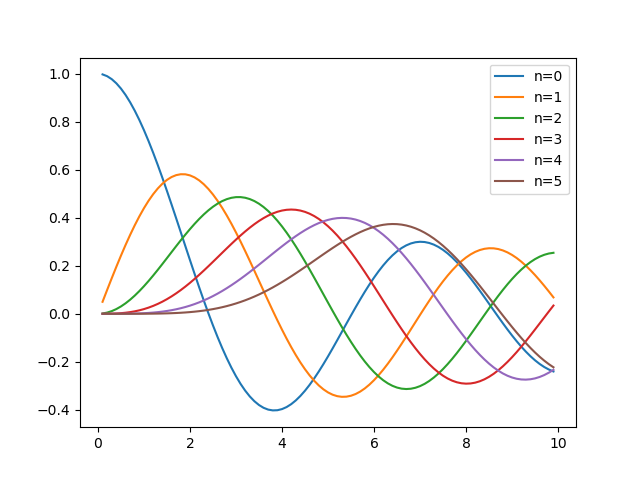
\includegraphics[width=\linewidth]{figures/BesselN.png}
	\caption{$n\in [0,5],x>0$时,Bessel函数的图形。$x<0$的图形可以由奇偶性得到。}
	\label{fig:figa}
	\end{subfigure}
	\hspace{20pt}   % Space between the figures
	\begin{subfigure}[b]{0.4\linewidth} % Fig (b)
		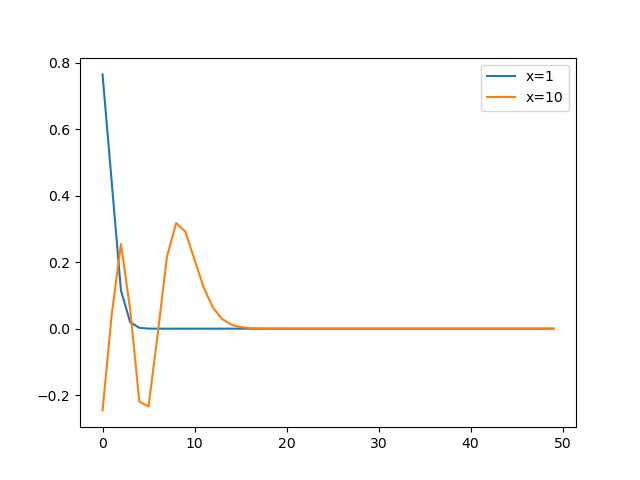
\includegraphics[width=\linewidth]{figures/BesselX.png}
		\caption{$x\in\{1,10\},n>0$时,Bessel函数的图形。}
		\label{fig:figb}
	\end{subfigure}
	\caption{$J_n(x)$是一个具有无穷个零点的衰减震荡函数。 \cite{PFGPlots}}
	\label{fig:examplefloat}
\end{figure*}
\subsection{Python Codes}
	\nolinenumbers
	\lstinputlisting[caption=code, language=Matlab]{main.py}
	\linenumbers
%\clearpage%新一页而不是新一列

	
%    If line numbering is enabled, we recommend placing the command \verb|\nolinenumbers| at the beginning %and \verb|\linenumbers| at the end of the code. 
%	
%    This will temporarily remove line numbering and the code will look better as shown in this example.

%----------------------------------------------------------

\addcontentsline{toc}{section}{References}

\printbibliography

%----------------------------------------------------------
%\section{Document style options}
%
%    \subsection{Tau start}
%	
%        We included the \verb|\taustart{}| command, which provides a personalized lettrine for the %beginning of a paragraph.
%
%    \subsection{Line numbering}
%	
%        By implementing the \textit{lineno} package, the line numbering of the document can be placed with %the command \verb|\linenumbers|.
%		
%        I recommend placing the command after the abstract and table of contents for a better appearance.
%		
%    \subsection{Table of contents}
%	
%        The \textit{tau class} provides a customised design for the table of contents. Each level of the %ToC provides a preview of the content and its location in the document. 
%		
%section{Figures and tables}
%
%   \subsection{Figures}
%		
%	Fig. \ref{fig:figure} shows an example figure.
%		
%	\begin{figure}[H]
%		\centering
%		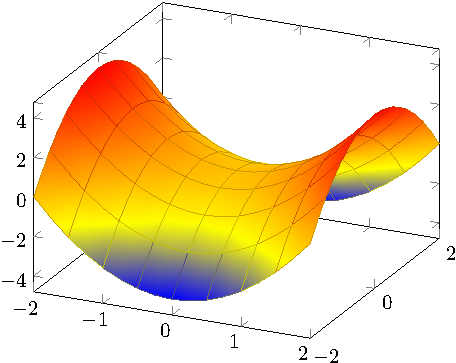
\includegraphics[width=0.75\columnwidth]{figures/Example.pdf}
%		\caption{Example figure obtained from PGFPlots \cite{PFGPlots}.}
%		\label{fig:figure}
%	\end{figure}
%		
%       Fig. \ref{fig:examplefloat} shows an example of two figures that covers the width of the page. It can be placed at the top or bottom of the page. The space between the figures can also be changed using the \verb|\hspace{Xpt}| command.
%		
   
	
%    \subsection{Tables}
%	
%        Table \ref{tab:table} shows an example table. The \verb|\tabletext{}| is used to add notes to %tables easily. 
%		
%	\begin{table}[H]
%		\centering
%		\caption{Small example table.}
%		\label{tab:table}
%		\begin{tabular}{cc}
%			\toprule
%			\textbf{Column 1} & \textbf{Column 2} \\
%			\midrule
%			Data 1 & Data 2 \\
%			Data 3 & Data 4 \\
%			\bottomrule
%		\end{tabular}
%			
%            \tabletext{Note: I'm a table text for additional information.}
%			
%	\end{table}
%		
%\section{Tau packages}
%
%    \subsection{Tauenvs}
%	
%		
%	\begin{tauenv}[frametitle=Environment with custom title]
%            This is an example of the custom title environment. To add a title type \verb|[frametitle=Your %title]| next to the beginning of the environment (as shown in this example).
%	\end{tauenv}
%
%		
%\section{Equation}
%
%    Equation \ref{ec:equation}, shows the Schrödinger equation as an example. 
%	\begin{equation} \label{ec:equation}
%		\frac{\hbar^2}{2m}\nabla^2\Psi + V(\mathbf{r})\Psi = -i\hbar \frac{\partial\Psi}{\partial t}
%	\end{equation} 
\end{document}